%%%%%%%%%%%%%%%%%%%%%%%%%%%%%%%%%%%%%%%%%%%%%%%%
%% Compile the master file!
%% 		Slides: Antonio Machicao y Priemer
%% 		Course: Wissenschaftliches Arbeiten
%%%%%%%%%%%%%%%%%%%%%%%%%%%%%%%%%%%%%%%%%%%%%%%%


%%%%%%%%%%%%%%%%%%%%%%%%%%%%%%%%%%%%%%%%%%%%%%%%%%%%
%%%             Metadata                        
%%%%%%%%%%%%%%%%%%%%%%%%%%%%%%%%%%%%%%%%%%%%%%%%%%%%      

\title{
	Wissenschaftliches Arbeiten in der Linguistik\\
	(Technische Übung)
}

\subtitle{\LaTeX\ 3: Umgebungen \& Verweise}

\author[aMyP]{
	{\small Antonio Machicao y Priemer (Vertretung: Felix Kopecky)}
	\\
	{\footnotesize \url{http://www.linguistik.hu-berlin.de/staff/amyp}}
%	\\
%	{\footnotesize \href{mailto:mapriema@hu-berlin.de}{mapriema@hu-berlin.de}}
}

\institute{Institut für deutsche Sprache und Linguistik}
 
%\date{ }

%\publishers{\textbf{6. linguistischer Methodenworkshop \\ Humboldt-Universität zu Berlin}}

%\hyphenation{nobreak}


%%%%%%%%%%%%%%%%%%%%%%%%%%%%%%%%%%%%%%%%%%%%%%%%%%%%
%%%             Preamble's End                  
%%%%%%%%%%%%%%%%%%%%%%%%%%%%%%%%%%%%%%%%%%%%%%%%%%%%      


%%%%%%%%%%%%%%%%%%%%%%%%%%%%%%%%%%
%%%%%%%%%%%%%%%%%%%%%%%%%%%%%%%%%%
%% Title slide 
\begin{frame}
	\HUtitle
\end{frame}


%% Contents slide
\frame{
\begin{multicols}{2}
	\frametitle{Inhaltsverzeichnis}
%	\tableofcontents[hideallsubsections]
	\tableofcontents
	%[pausesections]
\end{multicols}
	}

%%%%%%%%%%%%%%%%%%%%%%%%%%%%%%%%%%%%
%%%%%%%%%%%%%%%%%%%%%%%%%%%%%%%%%%%%
%% Extra literature

\nocite{Freitag&MyP15a}
\nocite{Knuth1986}
\nocite{Kopka94a}
\nocite{MyP17c}
\nocite{MyP&Kerkhof16a}
	
%%%%%%%%%%%%%%%%%%%%%%%%%%%%%%%%%%%%
%%%%%%%%%%%%%%%%%%%%%%%%%%%%%%%%%%%%


%%%%%%%%%%%%%%%%%%%%%%%%%%%%%%%%%%%%
%%%%%%%%%%%%%%%%%%%%%%%%%%%%%%%%%%%%
%%% Basic literature for these slides

\begin{frame}
\frametitle{Grundlage \& empfohlene Lektüre}

\dots basierend auf \citet{Freitag&MyP15a} und 

auf \citet{MyP&Kerkhof16a}\\
\ras \href{https://www.researchgate.net/publication/279514740_LATEX-Einfuhrung_fur_Linguisten}{LINK}

\end{frame}


%%%%%%%%%%%%%%%%%%%%%%%%%%%%%%%%%%%
%%%%%%%%%%%%%%%%%%%%%%%%%%%%%%%%%%%
\section{Nicht-textbezogene Elemente}
\frame{
	\frametitle{~}
	\begin{multicols}{2}
		\tableofcontents[currentsection,hideallsubsections]
	\end{multicols}
}
%%%%%%%%%%%%%%%%%%%%%%%%%%%%%%%%%%%

\begin{frame}
\frametitle{Nicht-textbezogene Elemente}

\begin{itemize}
	\item Grafiken
	
	\item Tabellen
	
	\item Gleitumgebungen (auch \gqq{floats} genannt)
	
	\item Abbildungs- und Tabellenverzeichnis	
	
\end{itemize}
\end{frame}


%%%%%%%%%%%%%%%%%%%%%%%%%%%%%%%%%%
%%%%%%%%%%%%%%%%%%%%%%%%%%%%%%%%%%
\subsection{Grafiken}
%\frame{
%\begin{multicols}{2}
%\frametitle{~}
%	\tableofcontents[currentsection]
%\end{multicols}
%}
%%%%%%%%%%%%%%%%%%%%%%%%%%%%%%%%%%

\begin{frame}[fragile]
\frametitle{Grafiken}

\begin{itemize}
	\item \LaTeX\ erlaubt sowohl das \textbf{Einfügen von externen Grafiken}, als auch das \textbf{Generieren eigener Grafiken}.
	
	(In diesem Kurs werden \ras nur Einfügen externer Grafiken)
	
	\item Um Grafiken einzufügen, muss das \textbf{Paket} \ltxterm{graphicx} in der Präambel mit dem folgenden Befehl geladen werden: 
	
\begin{lstlisting}
\usepackage{graphicx}
\end{lstlisting}

	\item Anschließend können mit dem \textbf{Befehl} \ltxterm{includegraphics} und der folgenden \textbf{Syntax} Grafiken in das Dokument eingefügt werden:
	
\begin{lstlisting}
\includegraphics[Größe]{Pfad/Dateiname}  
\end{lstlisting}


\end{itemize}

\end{frame}


%%%%%%%%%%%%%%%%%%%%%%%%%%%%%%%%%%%
\begin{frame}[fragile]
\frametitle{Grafiken einfügen}

\noindent Ein konkretes Beispiel:

\begin{lstlisting}
\includegraphics{LaTeX-flowchart-1.pdf}    
\end{lstlisting}

\includegraphics{../../texfiles-beamer/tex-material/WissArb-latex/LaTeX-flowchart-1.pdf}   

(Die \textbf{Dateiendung} \ltxpack{.pdf} muss \idR nicht angegeben werden.) 

\end{frame}


%%%%%%%%%%%%%%%%%%%%%%%%%%%%%%%%%%%
\begin{frame}[fragile]
\frametitle{Skalieren der Grafiken}

Die Größe der Grafik im Dokument kann \textbf{relativ zur Originalgröße} der Grafik spezifiziert werden, wie in dem folgenden Beispiel:

\begin{lstlisting}
\includegraphics[scale=0.5]{LaTeX-flowchart-1.pdf}  
\end{lstlisting}

\includegraphics[scale=0.5]{../../texfiles-beamer/tex-material/WissArb-latex/LaTeX-flowchart-1.pdf}

\noindent Die Größenangabe \ltxterm{scale}\texttt{=0.5} meint, dass die Größe der Grafik im Dokument 50\,\% von der Originalgröße betragen soll.\par

\end{frame}


%%%%%%%%%%%%%%%%%%%%%%%%%%%%%%%%%%%
\begin{frame}[fragile]
\frametitle{Skalieren der Grafiken}

Die Grafiken können auch mit \textbf{absoluten Größenangaben} geladen werden:

\begin{lstlisting}
\includegraphics[width=10cm]{LaTeX-flowchart-1.pdf}
\includegraphics[height=10cm]{LaTeX-flowchart-1.pdf}
\end{lstlisting}

oder mit Größen \textbf{relativ zur Dokumentengröße}:

\begin{lstlisting}
\includegraphics[width=\linewidth]{LaTeX-flowchart-1.pdf}  
\includegraphics[width=.2\linewidth]{LaTeX-flowchart-1.pdf}
\includegraphics[width=.2\textwidth]{LaTeX-flowchart-1.pdf}
\end{lstlisting}

%\includegraphics[width=.2\textwidth]{../../texfiles-beamer/tex-material/WissArb-latex/LaTeX-flowchart-1.pdf}

\includegraphics[width=.2\linewidth]{../../texfiles-beamer/tex-material/WissArb-latex/LaTeX-flowchart-1}
\end{frame}


%%%%%%%%%%%%%%%%%%%%%%%%%%%%%%%%%%%
\begin{frame}[fragile]
\frametitle{Formate}

Die folgenden Formate werden bei der Kompilierung (mit PDF-\LaTeX ) unterstützt:
\begin{itemize}
\item \ltxterm{.pdf}, Format für Vektorgrafiken
\item \ltxterm{.png}, Format für Rastergrafiken
\item \ltxterm{.jpg}, Format für Rastergrafiken
\item \ltxterm{.eps}, Format für Vektorgrafiken (nur mit dem \ltxterm{epstopdf}-Paket benutzbar)
\end{itemize}

\end{frame}


%%%%%%%%%%%%%%%%%%%%%%%%%%%%%%%%%%%
\begin{frame}[fragile]
\frametitle{Grafikpfad}

\begin{itemize}
	\item Wenn alle Grafiken \textbf{in einem Ordner} gesammelt werden (z.\,B. \texttt{graphics}), dann muss der Pfad zu diesem Ordner präzisiert werden.

	\item Der Weg zur Grafik ist immer \textbf{ausgehend vom Ort, an dem sich die kompilierte \ltxterm{.tex}-Datei befindet,} zu bestimmen.
\end{itemize}

\begin{lstlisting}
\includegraphics[scale=0.5]{graphics/LaTeX-flowchart-1.pdf}  
\end{lstlisting}
(Ordner \texttt{graphics} und \ltxterm{.tex}-Datei im gleichen Ordner)


\begin{itemize}
	\item Ist die Grafik außerhalb des Ordners, in dem sich die \ltxterm{.tex}-Datei befindet, dann kann man eine Ebene höher in der Ordnerstruktur mit dem \textbf{Präfix} \ltxterm{../} gelangen.
\end{itemize}

\begin{lstlisting}
\includegraphics[scale=0.5]{../LaTeX-flowchart-1.pdf}  
\end{lstlisting}


\end{frame}


%%%%%%%%%%%%%%%%%%%%%%%%%%%%%%%%%%
%%%%%%%%%%%%%%%%%%%%%%%%%%%%%%%%%%
\subsection{Tabellen}
%\frame{
%\begin{multicols}{2}
%\frametitle{~}
%	\tableofcontents[currentsection]
%\end{multicols}
%}
%%%%%%%%%%%%%%%%%%%%%%%%%%%%%%%%%%

\begin{frame}[fragile]
\frametitle{Tabellen}

Im Grunde ist die Erstellung von Tabellen in \LaTeX\ sehr \textbf{einfach}, wenn auch \textbf{gewöhnungsbedürftig}. Die Umgebung für Tabellen heißt \ltxterm{tabular} und nimmt ein optionales und ein obligatorisches Argument.
\begin{lstlisting}
\begin{tabular}[Position]{Layout}
...    
\end{tabular}
\end{lstlisting}

\pause 

Ein Beispiel:

\begin{multicols}{2}
	
{\scriptsize
\begin{lstlisting}
\begin{tabular}[t]{|l|c|r|}
\hline
Zelle 01 & Zelle 02 & Zelle 03 \\
\hline
Zelle A & Zelle B & Zelle C \\
\hline
Zelle  & Zelle  & Zelle  \\
\hline
\end{tabular}
\end{lstlisting}
}
	
	\columnbreak
	
	%\scalebox{.8}{
\begin{tabular}[t]{|l|c|r|}
	\hline
	Zelle 01 & Zelle 02 & Zelle 03 \\
	\hline
	Zelle A & Zelle B & Zelle C \\
	\hline
	Zelle  & Zelle  & Zelle  \\
	\hline
\end{tabular}
	%}
\end{multicols}

\end{frame}


%%%%%%%%%%%%%%%%%%%%%%%%%%%%%%%%%%
\begin{frame}[fragile]
%\frametitle{Tabellen}
	
Die Option \textbf{Position} kann die Werte \ltxterm{t} (top), \ltxterm{c} (center), oder \ltxterm{b} (bottom) annehmen. 
Diese Positionswerte geben die \textbf{vertikale Positionierung der gesamten Tabelle in Bezug zur aktuellen Zeile} (zur zuletzt geschriebenen Zeile), die Default-Einstellung ist in diesem Fall \ltxterm{center}.

\begin{multicols}{2}

Code für \textbf{top}:
	
		\columnbreak
		
{\scriptsize
\begin{lstlisting}
Hier ist die aktuelle Zeile
\begin{tabular}[t]{l|c|r}
Zelle 01 & Zelle 02 & Zelle 03 \\
\hline
Zelle A & Zelle B & Zelle C \\
\hline
Zelle  & Zelle  & Zelle  \\
\end{tabular}
\end{lstlisting}
}
	
\end{multicols}
	
Hier ist die aktuelle Zeile	
	\begin{tabular}[t]{l|c|r}
		Zelle 01 & Zelle 02 & Zelle 03 \\
		\hline
		Zelle A & Zelle B & Zelle C \\
		\hline
		Zelle  & Zelle  & Zelle  \\
	\end{tabular}

\end{frame}


%%%%%%%%%%%%%%%%%%%%%%%%%%%%%%%%%%
\begin{frame}[fragile]
%\frametitle{Tabellen}

\begin{multicols}{2}
	
Code für \textbf{bottom}:
	
\columnbreak

{\tiny
\begin{lstlisting}
Hier ist die aktuelle Zeile
\begin{tabular}[b]{l|c|r}
Zelle 01 & Zelle 02 & Zelle 03 \\
\hline
Zelle A & Zelle B & Zelle C \\
\hline
Zelle  & Zelle  & Zelle  \\
\end{tabular}
\end{lstlisting}
}

\end{multicols}

Hier ist die aktuelle Zeile	
\begin{tabular}[b]{l|c|r}
	Zelle 01 & Zelle 02 & Zelle 03 \\
	\hline
	Zelle A & Zelle B & Zelle C \\
	\hline
	Zelle  & Zelle  & Zelle  \\
\end{tabular}


\pause 


\begin{multicols}{2}
	
Code für \textbf{center}:
	
\columnbreak

{\tiny
\begin{lstlisting}
Hier ist die aktuelle Zeile
\begin{tabular}[c]{l|c|r}
Zelle 01 & Zelle 02 & Zelle 03 \\
\hline
Zelle A & Zelle B & Zelle C \\
\hline
Zelle  & Zelle  & Zelle  \\
\end{tabular}
\end{lstlisting}
}

\end{multicols}


Hier ist die aktuelle Zeile	
\begin{tabular}[c]{l|c|r}
	Zelle 01 & Zelle 02 & Zelle 03 \\
	\hline
	Zelle A & Zelle B & Zelle C \\
	\hline
	Zelle  & Zelle  & Zelle  \\
\end{tabular}

\end{frame}


%%%%%%%%%%%%%%%%%%%%%%%%%%%%%%%%%%%
\begin{frame}[fragile]
%\frametitle{Tabellen}
Das obligatorische Argument \textbf{Layout} gibt Folgendes an:

\begin{itemize}
	\item Spaltenanzahl,
	
	\item Textausrichtung in den Spalten

	\item mögliche Werte:
	
	\begin{itemize}
		\item \ltxterm{l}: linksbündig
		\item \ltxterm{c}: Zentriert
		\item \ltxterm{r}: rechtsbündig
		\item \ltxterm{p\{length\}}: feste Breite
		\item \ltxterm{|} (pipe): vertikale Linien zwischen Spalten werden eingefügt
	\end{itemize}
	
\end{itemize}

\pause 

\begin{multicols}{2}
	
{\scriptsize
\begin{lstlisting}
\begin{tabular}[t]{|l|c|r|}
\hline
Zelle 1.1 & Zelle 1.2 & Zelle 1.3 \\
\hline
Zelle 2.1 & Zelle 2.2 & Zelle 2.3 \\
\hline
Zelle  & Zelle  & Zelle  \\
\hline
\end{tabular}
\end{lstlisting}
}
	
	\columnbreak
	
	%\scalebox{.8}{
	\begin{tabular}[t]{|l|c|r|}
		\hline
		Zelle 1.1 & Zelle 1.2 & Zelle 1.3 \\
		\hline
		Zelle 2.1 & Zelle 2.2 & Zelle 2.3 \\
		\hline
		Zelle  & Zelle  & Zelle  \\
		\hline
	\end{tabular}
	%}
\end{multicols}

\end{frame}


%%%%%%%%%%%%%%%%%%%%%%%%%%%%%%%%%%%
\begin{frame}[fragile]
%\frametitle{Tabellen}

\begin{itemize}
	\item Tabellen werden Zeile für Zeile geschrieben. 
	
	\item Das \textbf{Et-Zeichen} \ltxterm{\&} trennt zwei Zellen von einander.
	
	\item Der \textbf{doppelte Backslash} \textbackslash\textbackslash\ markiert das Ende einer Zeile.
	
\end{itemize}

\small{
\begin{lstlisting}
Aktuelle Zeile
\begin{tabular}[c]{lc|rp{1.7cm}|}
l-bündig & zentriert & r-bündig & feste Breite \\
\hline
viel Inhalt & viel Inhalt & viel viel Inhalt & viel viel Inhalt \\
wenig & & wenig & wenig \\
\end{tabular}
\end{lstlisting}

%\outputbox{
Aktuelle Zeile
\begin{tabular}[c]{lc|rp{1.7cm}|}
	l-bündig & zentriert & r-bündig & feste Breite \\
	\hline
viel Inhalt & viel Inhalt & viel viel Inhalt & viel viel Inhalt \\
	wenig & & wenig & wenig \\
\end{tabular}
}
%}
\end{frame}


%%%%%%%%%%%%%%%%%%%%%%%%%%%%%%%%%%%
\begin{frame}[fragile]
%\frametitle{Tabellen}

\footnotesize{
Beispiele weiterer Tabellen:

\begin{multicols}{2}

\begin{tabular}[t]{llr}
\multicolumn{2}{c}{Item} &  \\
article & unit & price \\
proofreading & per words & 0.02 \\
layout & per page & 0.80 \\
printing & per page & 0.99 \\
typesetting & per article & 40.33 \\
\end{tabular}

\vspace{\baselineskip}

\begin{tabular}[t]{|l|l|r|}
\hline
\multicolumn{2}{|c}{Item} &  \\
\hline
article & unit & price \\
\hline
proofreading & per words & 0.02 \\
\hline
layout & per page & 0.80 \\
\hline
printing & per page & 0.99 \\
\hline
typesetting & per article & 40.33 \\
\hline
\end{tabular}

\vspace{\baselineskip}

\columnbreak{}

\begin{tabular}[t]{llr}
\hline
\multicolumn{2}{c}{Item} &  \\
\cline{1-2}
article & unit & price \\
\hline
proofreading & per words & 0.02 \\
layout & per page & 0.80 \\
printing & per page & 0.99 \\
typesetting & per article & 40.33 \\
\hline
\end{tabular}

\vspace{\baselineskip}

\begin{tabular}[t]{llr}
\toprule
\multicolumn{2}{c}{Item} &  \\
\cmidrule{1-2}
article & unit & price \\
\midrule
proofreading & per words & 0.02 \\
layout & per page & 0.80 \\
printing & per page & 0.99 \\
typesetting & per article & 40.33 \\
\bottomrule
\end{tabular}

\end{multicols}
}
\end{frame}


%%%%%%%%%%%%%%%%%%%%%%%%%%%%%%%%%%%
%%%%%%%%%%%%%%%%%%%%%%%%%%%%%%%%%%
\subsection{Gleitumgebung}
\label{sec:floating}
%\frame{
%\begin{multicols}{2}
%\frametitle{~}
%	\tableofcontents[currentsection]
%\end{multicols}
%}
%%%%%%%%%%%%%%%%%%%%%%%%%%%%%%%%%%

\begin{frame}[fragile]
\frametitle{Gleitumgebung}

\begin{itemize}
	
	\item Bilder und Tabellen können \textbf{sehr viel Platz} auf einer Seite einnehmen.
	
	\item[]
	
	\item Mit Hilfe von \textbf{Gleitumgebungen} verschiebt \LaTeX\ das Bild  bzw.\ die Tabelle an den günstigsten Platz, um \textbf{große Lücken in der Seitengestaltung} zu vermeiden.
	
	\ras wichtig aus typographischen Gründen!
	
\end{itemize}
\end{frame}


%%%%%%%%%%%%%%%%%%%%%%%%%%%%%%%%%%
\begin{frame}[fragile]
%\frametitle{Gleitumgebung}

{\small
\begin{lstlisting}
Hier das Beispiel dazu:
\begin{table}[htbp]
\centering
%  \caption[Beschriftung oben]{Lange Beschriftung oben 
%  (auskommentiert)}

\begin{tabular}[t]{ll}
\hline
Eins & Zwei \\
Drei & Vier \\
\hline
\end{tabular}

\caption[Beschriftung unten]{Lange Beschriftung unten}
\label{tab:beispiel-tabelle1}
\end{table}
\end{lstlisting}
}

\end{frame}


%%%%%%%%%%%%%%%%%%%%%%%%%%%%%%%%%%%
\begin{frame}[fragile]
%\frametitle{Gleitumgebung}

Hier das Beispiel dazu:
\begin{table}[htbp]
\centering
%  \caption[Beschriftung oben]{Lange Beschriftung oben 
%  (auskommentiert)}

\begin{tabular}[t]{ll}
	\hline
	Eins & Zwei \\
	Drei & Vier \\
	\hline
\end{tabular}

\caption[Beschriftung unten]{Lange Beschriftung unten}
\label{tab:beispiel-tabelle1}
\end{table}

\end{frame}


%%%%%%%%%%%%%%%%%%%%%%%%%%%%%%%%%%%
\begin{frame}[fragile]
%\frametitle{Gleitumgebung}

Das gleiche gilt auch für Grafiken, wie das folgende Beispiel zeigt:
\begin{lstlisting}
\begin{figure}[htbp]
\centering
\includegraphics[scale=0.5]{LaTeX-flowchart-1.pdf}
\caption{Durchlaufplan in \LaTeX }
\label{fig:latex-flowchart}
\end{figure}
\end{lstlisting}

\begin{figure}[htbp]
\centering
\includegraphics[scale=0.5]{../../texfiles-beamer/tex-material/WissArb-latex/LaTeX-flowchart-1.pdf}
\caption{Durchlaufplan in \LaTeX }
\label{fig:latex-flowchart}
\end{figure}

\end{frame}


%%%%%%%%%%%%%%%%%%%%%%%%%%%%%%%%%%
%%%%%%%%%%%%%%%%%%%%%%%%%%%%%%%%%%
\subsection{Abbildungs- und Tabellenverzeichnis}
%\frame{
%\begin{multicols}{2}
%\frametitle{~}
%	\tableofcontents[currentsection]
%\end{multicols}
%}
%%%%%%%%%%%%%%%%%%%%%%%%%%%%%%%%%%

\begin{frame}[fragile]
\frametitle{Abbildungs- und Tabellenverzeichnis}

\textbf{Abbildungs-} und \textbf{Tabellenverzeichnisse} werden einfach mit den folgenden Befehlen automatisch erstellt:

\begin{itemize}
	\item \lstinline|\listoffigures| \index{listoffigures}
	\item \lstinline|\listoftables| \index{listoftables}
\end{itemize}

Dieser Befehl soll an der \textbf{Position} im Dokument stehen, an der das entsprechende Verzeichnis im Output erscheinen soll (\idR nach dem Inhaltsverzeichnis). \LaTeX\ sammelt automatisch die Informationen aus den \textbf{\ltxterm{caption}-Informationen}.  
\end{frame}


%%%%%%%%%%%%%%%%%%%%%%%%%%%%%%%%%%
%%%%%%%%%%%%%%%%%%%%%%%%%%%%%%%%%%
\section{Querverweise}
\label{sec:references}
\frame{
	\frametitle{~}
	\begin{multicols}{2}
		\tableofcontents[currentsection,hideallsubsections]
	\end{multicols}
}


%%%%%%%%%%%%%%%%%%%%%%%%%%%%%%%%%%
%%%%%%%%%%%%%%%%%%%%%%%%%%%%%%%%%%
\subsection{Einfache Querverweise}
%\frame{
%\begin{multicols}{2}
%\frametitle{~}
%	\tableofcontents[currentsection]
%\end{multicols}
%}
%%%%%%%%%%%%%%%%%%%%%%%%%%%%%%%%%%

\begin{frame}[fragile]
\frametitle{Einfache Querverweise}

Mit \LaTeX\ ist es sehr einfach mit Querverweisen zu arbeiten. Es sind nur zwei Sachen dafür notwendig:

\begin{description}
	\item[Anker:] Dafür wird der Befehl \lstinline|\label{ID}| verwendet. 
	
	Die \ltxterm{ID} muss natürlich \textbf{einzigartig im Dokument} sein.
	
	\item[]
	
	\item[Verweis:] Dafür wird der Befehl \lstinline|\ref{ID}| benutzt, damit wird auf die (Beispiel-, Ab\-bil\-dungs- oder Tabellen-) \textbf{Nummer} verwiesen. 
	
	Mit dem Befehl \lstinline|\pageref{ID}| wird dagegen auf die \textbf{Seitenzahl} verwiesen, in der sich das Element befindet.
\end{description}

\end{frame}

%%%%%%%%%%%%%%%%%%%%%%%%%%%%%%%%%%%
\begin{frame}[fragile]
%\frametitle{Einfache Querverweise}

\begin{itemize}
	\item Das \ltxterm{label} muss immer \textbf{dem logischen Textauszeichnungsbefehl folgen}, auf das es sich bezieht (\zB \ltxterm{section}, \ltxterm{item}, \ltxterm{caption}, \dots). 
	\item[]
	
	\item Um Probleme zu vermeiden, empfiehlt es sich das \ltxterm{label} immer \textbf{unmittelbar} nach dem Textauszeichnungsbefehl zu positionieren.
	\item[]
	
	\item Wenn \LaTeX\ die \ltxterm{ID} des Eintrags \textbf{nicht findet}, weil man sich vielleicht verschrieben hat, wird statt des Verweises ein doppeltes Fragezeichen \ltxterm{??} stehen.  

\end{itemize}
%
\end{frame}

%%%%%%%%%%%%%%%%%%%%%%%%%%%%%%%%%%
%%%%%%%%%%%%%%%%%%%%%%%%%%%%%%%%%%
\subsection{Präfixe}
%\frame{
%\begin{multicols}{2}
%\frametitle{~}
%	\tableofcontents[currentsection]
%\end{multicols}
%}
%%%%%%%%%%%%%%%%%%%%%%%%%%%%%%%%%%

\begin{frame}[fragile]
\frametitle{Präfixe}

Präfixe bei den IDs helfen dabei die IDs in größeren Arbeiten schneller zu finden. 

\begin{description}
\item[\ltxterm{sec}] für alle Überschriften
\item[\ltxterm{cha}/\ltxterm{chap}] nur für Kapitel (\ltxterm{sec} kann auch benutzt werden)
\item[\ltxterm{part}] nur für Bücher, die auch in Teile gegliedert sind (\ltxterm{sec} kann auch benutzt werden)
\item[\ltxterm{fig}] für Abbildungen
\item[\ltxterm{tab}] für Tabellen
\item[\ltxterm{item}/\ltxterm{it}] für Listenpunkte
\item[\ltxterm{eqn}] für Gleichungen
\item[\ltxterm{fn}] für Fußnoten
\end{description}

\end{frame}

%%%%%%%%%%%%%%%%%%%%%%%%%%%%%%%%%%%
\begin{frame}[fragile]
%\frametitle{Präfixe}


{\small 
	
\begin{lstlisting}
Hier ist ein Querverweis auf die 
Tabelle~\ref{tab:beispiel-tabelle2}, die nach diesem Text kommt. 
Außerdem zeigen wir einen Verweis auf die 
Tabelle~\ref{tab:beispiel-tabelle1} auf 
Seite~\pageref{tab:beispiel-tabelle1} 
im Abschnitt~\ref{sec:floating}.

\begin{table}[htbp]
\centering
\begin{tabular}{lll}
Eins & Zwei & Drei \\
Vier & Fünf & Sechs\\
\end{tabular}
\caption{Beispieltabelle für Querverweise}
\label{tab:beispiel-tabelle2}
\end{table}
\end{lstlisting}
%\vspace{1em}
}
\end{frame}


%%%%%%%%%%%%%%%%%%%%%%%%%%%%%%%%%%%
\begin{frame}[fragile]
%\frametitle{Präfixe}



	Hier ist ein Querverweis auf die 
	Tabelle~\ref{tab:beispiel-tabelle2}, die nach diesem Text kommt. 
	Außerdem zeigen wir einen Verweis auf die 
	Tabelle~\ref{tab:beispiel-tabelle1} auf 
	Seite~\pageref{tab:beispiel-tabelle1} 
	im Abschnitt~\ref{sec:floating}.
	
	\begin{table}[htbp]
	\centering
	\begin{tabular}{lll}
	Eins & Zwei & Drei \\
	Vier & Fünf & Sechs\\
	\end{tabular}
	\caption{Beispieltabelle für Querverweise}
	\label{tab:beispiel-tabelle2}
	\end{table}

\end{frame}


%%%%%%%%%%%%%%%%%%%%%%%%%%%%%%%%%%%
\begin{frame}[fragile]
%\frametitle{Präfixe}

Finden Sie den Fehler:

{\small 
	
\begin{lstlisting}
Hier ist ein Querverweis auf die 
\alert{Tabelle~\ref{tab:beispiel-tabelle3}}, die nach diesem Text kommt. 

\begin{table}[htbp]
\begin{tabular}{lll}
Eins & Zwei & Drei \\
Vier & Fünf & Sechs\\
\end{tabular}
\caption{Beispieltabelle für Querverweise}
\end{table}
\label{tab:beispiel-tabelle3}
\end{lstlisting}
%\vspace{1em}
}

\vspace{1cm}

\pause 

Hier ist ein Querverweis auf die 
\alert{Tabelle~\ref{tab:beispiel-tabelle3}}, die nach diesem Text kommt. 

\begin{table}[htbp]
	\centering
	\begin{tabular}{lll}
		Eins & Zwei & Drei \\
		Vier & Fünf & Sechs\\
	\end{tabular}
	\caption{Beispieltabelle für Querverweise}
\end{table}

\label{tab:beispiel-tabelle3}

\end{frame}


%%%%%%%%%%%%%%%%%%%%%%%%%%%%%%%%%%
%%%%%%%%%%%%%%%%%%%%%%%%%%%%%%%%%%
\subsection{Querverweise als Links}
%\frame{
%\begin{multicols}{2}
%\frametitle{~}
%	\tableofcontents[currentsection]
%\end{multicols}
%}
%%%%%%%%%%%%%%%%%%%%%%%%%%%%%%%%%%

\begin{frame}[fragile]
\frametitle{Querverweise als Links}

\begin{itemize}
	\item Querverweise können in Dokumenten als \textbf{aktive Links} verwendet werden. 
	\item[]
	\item Dafür wird das \textbf{Paket \ltxterm{hyperref}} verwendet.
	
	\lstinline|\usepackage{hyperref}|
	
	\item[]	
	\item Mit der \textbf{Option \ltxterm{bookmarksnumbered}} wird bei der PDF ein nummeriertes Inhaltsverzeichnis generiert.
	
	\lstinline|\usepackage[bookmarksnumbered]{hyperref}|

	\item[]	
	\item Mit der \textbf{Option \ltxterm{hidelinks}} wird bei der PDF die Umrandung der Links unterbunden. Die farbige Umrandung der Links erscheint (ohne \ltxterm{hidelinks}) nur auf der PDF, nicht beim Druck! 
	
	\lstinline|\usepackage[bookmarksnumbered, hidelinks]{hyperref}|
\end{itemize}

\end{frame}


%%%%%%%%%%%%%%%%%%%%%%%%%%%%%%%%%%%
%%%%%%%%%%%%%%%%%%%%%%%%%%%%%%%%%%%
\section{Hausaufgabe 2}
\frame{
	%\frametitle{~}
	\begin{multicols}{2}
		\tableofcontents[currentsection,hideallsubsections]
	\end{multicols}
}
%%%%%%%%%%%%%%%%%%%%%%%%%%%%%%%%%%%

\begin{frame}[fragile]{Hausaufgabe 2: \LaTeX\ 2 \& 3}

\begin{itemize}
	
	\item Installieren Sie die folgenden Pakete in Ihrem \gqq{\texttt{myName.tex}}-Dokument (mit dem Befehl \ltxterm{usepackage}).
	
	\begin{itemize}
		\item \ltxterm{graphicx} 
		\item \ltxterm{blindtext}
		\item \ltxterm{hyperref}
		
		Installieren Sie \ltxterm{hyperref} mit der Option \ltxterm{bookmarksnumbered}. 
		
		Hier die Syntax dafür:
		
		\lstinline|\usepackage[bookmarksnumbered]{hyperref}|
		
	\end{itemize}

\end{itemize}

\end{frame}


%%%%%%%%%%%%%%%%%%%%%%%%%%%%%%%%%%%
\begin{frame}{Hausaufgabe 2: \LaTeX\ 2 \& 3}

\begin{itemize}

	\item Laden Sie die \texttt{pdf}-Dateien \gqq{\texttt{test2PDF.pdf}} und \gqq{\texttt{LaTeX-flowchart-1.pdf}} herunter.
	
	\item Verwenden Sie die \texttt{tex}-Datei \gqq{\texttt{myName.tex}} vom letzten Mal und
	
	\item geben Sie den benötigten Code ein, um das Ergebnis zu erhalten, das Sie in \gqq{\texttt{test2PDF.pdf}} sehen.
	
	\item Laden Sie dann Ihre \gqq{\texttt{myName.tex}}-Datei und Ihr PDF-Ergebnis bei Moodle hoch. 
	
	(nur die \alert{.tex-Datei} und die \alert{.pdf-Datei} -- KEINE HILFSDATEIEN)
	
	\item[NB:] Schauen Sie sich die Dokumentation des Pakets \ltxterm{blindtext} an, um zu sehen, wie Sie Text automatisch generieren können.
	
\end{itemize}

\end{frame}


%%%%%%%%%%%%%%%%%%%%%%%%%%%%%%%%%%%
\begin{frame}{Hausaufgabe -- Hinweise}

\begin{itemize}
	
	\item Es gibt Apps, mit denen Sie \LaTeX -Dokumente in Ihrem Smartphone schreiben können, \zB \ltxpack{VerbTeX LaTeX Editor}
	
	\item Die App \ltxpack{LaTeX Help} zeigt die Befehle für viele Sonderzeichen.
	
\end{itemize}

\end{frame}


%%%%%%%%%%%%%%%%%%%%%%%%%%%%%%%%%%%
%%%%%%%%%%%%%%%%%%%%%%%%%%%%%%%%%%%
%\section{XY}
%%\frame{
%%\begin{multicols}{2}
%%\frametitle{~}
%%	\tableofcontents[currentsection]
%%\end{multicols}
%%}
%%%%%%%%%%%%%%%%%%%%%%%%%%%%%%%%%%%
%
%\begin{frame}{XY}
%
%\begin{itemize}
%	\item XY
%\end{itemize}
%
%\end{frame}


%%%%%%%%%%%%%%%%%%%%%%%%%%%%%%%%%%%%
%%%%%%%%%%%%%%%%%%%%%%%%%%%%%%%%%%%%
%\iftoggle{handout}{
%	
%%%%%%%%%%%%%%%%%%%%%%%%%%%%%%%%%%%%%
%\begin{frame}
%%\frametitle{Bücher \& Artikel}
%	
%Test Toggle ON
%	
%\end{frame}
%
%}
%%% END handout true 
%%% BEGIN handout false
%{
%%%%%%%%%%%%%%%%%%%%%%%%%%%%%%%%%%%
%
%%% EMPTY
%
%}%% END HO-Toggle
%%%%%%%%%%%%%%%%%%%%%%%%%%%%%%%%%%%